\chapter{Contesto}
%In questo capitolo vengono spiegate le tecnologie adottate. %TODO
%I suggest referencing stuff as follows: \cref{fig:random-image} or \Cref{fig:random-image}

\section{Alchemist}
Alchemist\space\cite{Pianini_2013} è un simulatore DES (Discrete Event System) che estende il modello computazionale 
base delle reazioni chimiche in modo tale da favorirne l'applicabilità a situazioni complesse,
pur mantenendo elevate prestazioni. In particolare, Alchemist si fonda su una versione ottimizzata 
dell'algoritmo di Gillespie\cite{gillespie1977exact} chiamata Next Reaction Method\cite{gibson2000efficient}, esteso in modo tale da poter lavorare 
con un ambiente agile e dinamico dove è possibile aggiungere o rimuovere reazioni, dati e
connessioni topologiche. Le applicazioni già implementate sono varie e comprendono, ad esempio, 
simulazioni di reazioni biochimiche e movimento di pedoni. Il punto di forza del sistema è il 
meta-modello estremamente astratto, la cui effettiva realizzazione è demandata alle ``incarnazioni'',
le quali rappresentano l'implementazione vera e propria delle diverse categorie di simulazioni 
eseguibili all'interno. Attualmente troviamo 4 incarnazioni: 
\begin{itemize}
    \item Protelis
    \item SAPERE
    \item Biochemistry
    \item Scafi
\end{itemize}
\subsection{Il meta-modello} 
Come accennato in precedenza, il meta-modello è uno dei punti di forza maggiori di Alchemist. 
Per meta-modello si intende un tipo di paradigma che descrive la struttura, le regole e le relazioni
che i modelli di dati devono seguire all'interno di un sistema. Rappresenta in modo astratto i 
concetti e le relazioni all'interno del dominio di interesse e stabilisce i vincoli e le convenzioni
che tutti i modelli devono usare. Dunque, tutte le incarnazioni sviluppate presentano le stesse entità
``base''. Poichè Alchemist è sviluppato partendo da un'ispirazione orientata alla chimica/biochimica,
le entità presentano nomi riconducibili a quei mondi. Infatti troviamo:
\begin{itemize}
    \item \textbf{Molecole} (\textit{molecule}): il nome di un dato, concettualmente interpretabile come il nome di una variabile.
    \item \textbf{Concentrazioni} (\textit{concentration}): il valore associato alla molecola.
    \item \textbf{Nodi}\label{node} (\textit{node}): il ``contenitore'' di molecole e reazioni.
    \item \textbf{Ambiente} (\textit{environment}): l'astrazione dello spazio; è un “contenitore” di nodi e svolge i seguenti compiti:
    \begin{itemize}
        \item Restituire la posizione dei nodi.
        \item Restituire la distanza tra due nodi.
        \item Supportare il movimento dei nodi, se presente.
    \end{itemize}
    \item \textbf{Vicinato} (\textit{neighborhood}): un entità composta da un nodo centrale e un insieme di nodi vicini.
    \item \textbf{Regola di collegamento} (\textit{linking rule}): una funzione relativa allo stato corrente dell'ambiente che associa ad ogni nodo un vicinato.
    \item \textbf{Reazione} (\textit{reaction}): un qualsiasi evento che provoca un cambiamento dello stato dell'ambiente. È definita da una lista di condizioni, una o più lista di azioni e una distribuzione temporale. La frequenza con la quale avviene una reazione dipende da:
    \begin{itemize}
        \item Un parametro statico ``rate''.
        \item Il valore di ogni condizione.
        \item Una ``rate equation'', ovvero una equazione che combina il parametro statico (rate) con i valori delle condizioni, restituendo un ``instantaneous rate''.
        \item Una distribuzione temporale.
    \end{itemize}
    \item \textbf{Condizione} (\textit{condition}): una funzione che, dato lo stato attuale del'ambiente (environment), restituisce un booleano ed un numero. Se il booleano è falso la reazione non può avvenire. In caso contrario, invece, avviene. Il numero può invece influenzare la velocità della reazione a seconda della reazione e della distribuzione temporale.
    \item \textbf{Azione} (\textit{action}): un cambiamento nell'ambiente.
\end{itemize}

\begin{figure}[ht]
    \centering
    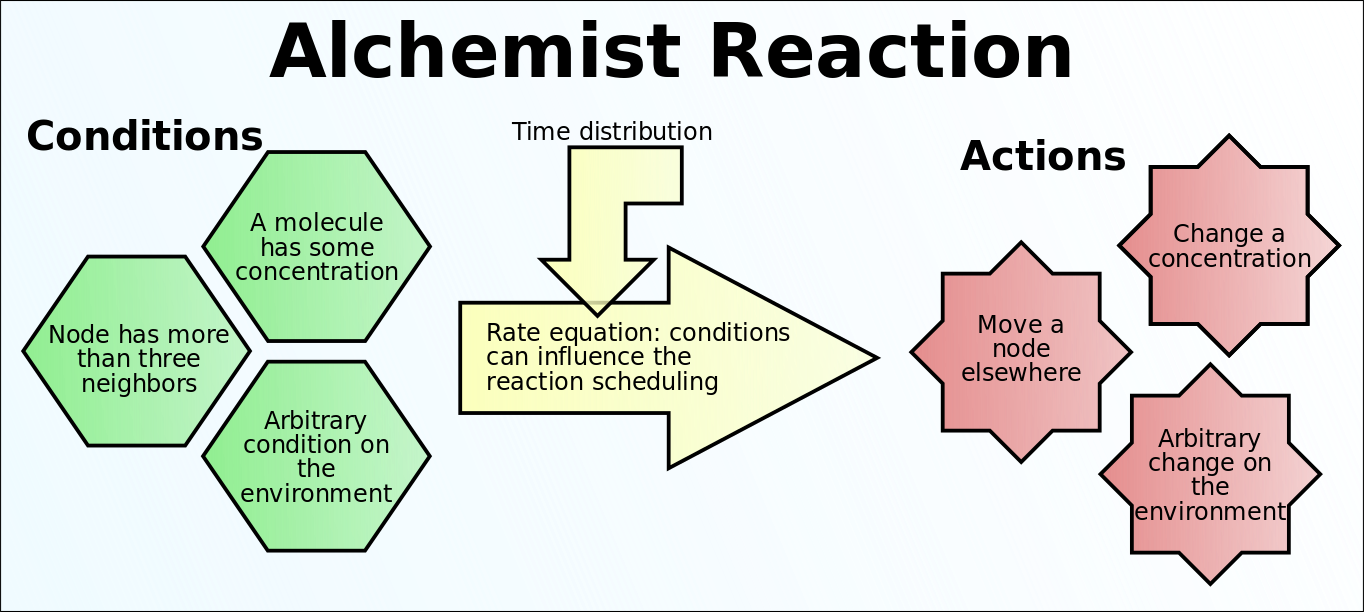
\includegraphics[width=.8\linewidth]{figures/alchemistReaction.png}
    \caption{Rappresentazione di una reazione in Alchemist}\label{fig:reactionAlchemist}
\end{figure}
\begin{figure}[ht]
    \centering
    \includegraphics[width=.8\linewidth]{figures/alchemistModel.png}
    \caption{Il modello di Alchemist}\label{fig:rmodelAlchemist}
\end{figure}
\clearpage

\section{Simulazione di riferimento}\label{refSim}
La simulazione utilizzata come riferimento per questo progetto di tesi è presente nella libreria
di modelli di NetLogo\space\cite{wilensky1997netlogo}. Il modello di riferimento è ``Slime``\space\cite{wilensky1997netlogo}
e per simulare l'aggregazione di tanti singoli organismi in un gruppo si fa riferimento al comportamento delle tartarughe.
Quest'ultime si muovono in uno spazio a griglia e durante il loro movimento rilasciano una particolare molecola
chiamata ``feromone'' che si deposita in una posizione precisa. L'intero mondo è quindi suddiviso
in tantissime ``micro-aree'' chiamate \textit{patch}. La tartaruga per muoversi 
``annusa'' davanti a se, ovvero percepisce se nelle \textit{patch} vicine è presente del ``feromone''. Se il valore di quest'ultimo è abbastanza alto, la 
tartaruga si sposterà nella posizione ``annusata'', mentre, in caso contrario la tartaruga si muoverà in modo randomico nello spazio circostante. 
Durante tutto ciò, le \textit{patches} diffonderanno del ``feromone'' alle varie posizioni vicine e, con il passare del tempo,
il ``feromone'' tende ad evaporare (ovvero sparire) dalla griglia.
\begin{figure}[ht]
    \centering
    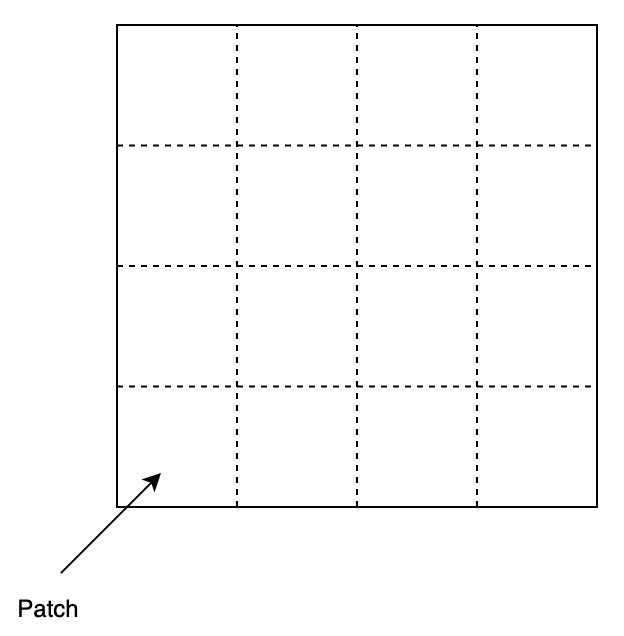
\includegraphics[width=.6\linewidth]{figures/patch.png}
    \caption{Il mondo suddiviso in patch}\label{fig:patch}
\end{figure}
\clearpage
\section{Overview su \textit{slime-mold}}
Nel contesto della presente tesi, sulla base della simulazione di riferimento\ref{refSim} e i comportamenti osservati in essa, si è scelto di indagare un altro 
fenomeno dalle caratteristiche estremamente simili: la muffa mucillaginosa.
In natura, l'aggregazione delle cellule di muffa mucillaginosa (detti anche funghi mucillaginosi o, in inglese, \textit{slime-mold}) rappresenta
comportamento in cui entità individuali interagiscono tra di loro per formare strutture complesse e funzionali. 
Lo \textit{slime-mold} è un organismo unicellulare ma, talvolta, può trovarsi anche ad agire come un'entità multicellulare. 
Pur non essendo un fungo è spesso classificato nella stessa categoria per via delle sue caratteristiche affini a quelle di questi organismi.
La particolarità principale della muffa mucillaginosa è che può comportarsi come un organismo unicellulare o multicellulare a seconda delle diverse 
condizioni ambientali in cui si trova.
L'habitat principale di questi organismi è il terreno umido, dove di solito si nutrono di foglie morte o di tronchi di alberi in putrefazione.
Quando trova una fonte di cibo, lo \textit{slime-mold} si aggrega, formando una massa citoplasmatica detta ``plasmodio'', composta da un grande numero cellule. Inoltre,
questa massa può muoversi, ``navigando'' attraverso il terreno in cerca di cibo.
Infatti, se le risorse alimentari scarseggiano o l'ambiente diventa meno ospitale, lo \textit{slime-mold} può assumere forme diverse: può formare spore, 
resistenti per sopravvivere in condizioni avverse, oppure aggregarsi insieme ad altri individui simili per formare una struttura multicellulare
che si comporta come un'unica entità, condividendone di conseguenza risorse e compiti.
